\chapter{Szövegfüggvények}
\thispagestyle{empty}

Ebben a kategóriában több tucat függvényt találunk, amelyek
segítségével szövegtartalmú cellákkal végezhetünk
különböző műveleteket.

A \textbf{CONCATENATE} függvény segítségével egyetlen
karakterlánccá egyesíthetjük az  argumentumban megadott
karakterláncokat. Az argumentumok lehetnek cellahivatkozások is.

Az \textbf{EXACT} összehasonlít két szöveges karakterláncot.
Amikor azok megegyeznek, IGAZ értéket ad vissza. Ez a függvény
különbséget tesz kis- és nagybetűk között.

A \textbf{SEARCH} függvény egy szövegrész karakterláncon
belüli helyzetét adja eredményül. A keresés
kezdőpontját paraméterként adhatja meg.  A keresés nem
különbözteti meg a kis- és nagybetűket. A
SEARCH("m";"Mamut")
eredménye 1 lesz, mert a Mamut szó első karaktere  m.

A \textbf{FIND} függvény szöveget keres egy másikban, és
megadja, hogy hányadik karaktertől kezdődik. Opcionális
paraméterként megadható, hogy a keresés melyik karaktertől
kezdődjön. A keresés megkülönbözteti a kis- és
nagybetűket. A
FIND("m";"Mamut")
eredménye 3 lesz, mert a kis m betű harmadik a Mamut szóban.

A \textbf{LEFT} függvény egy szöveg első karaktereit adja
eredményül. A LEFT("rendszer";4) eredménye a ,,rend'' szó lesz. A második
paramétert el is hagyhatjuk, ilyenkor csak az első karaktert adja
eredményül.

A \textbf{RIGHT} függvénnyel egy szöveg utolsó karaktereit
jeleníthetjük meg. A RIGHT("alma";2) eredménye a ,,ma'' szó lesz.

A \textbf{MID} függvény egy karakterlánc egy darabját adja
vissza. A kezdőpozíciót, illetve a karakterek számát a
paraméterek határozzák meg. A MID("karaktereit";4;3)
eredménye az ,,akt'' szó lesz.

A \textbf{LEN} függvény egy szövegnek a szóközökkel együtt
vett hosszát adja eredményül.

A \textbf{LOWER} függvény argumentumában megadott szöveg minden
nagybetűjét kisbetűre cseréli.

A \textbf{PROPER} függvény nagybetűsre változtatja egy
szöveg minden szavának első betűjét.

Az \textbf{UPPER} függvény argumentumában megadott szöveg minden
kisbetűjét nagybetűre cseréli.

A \textbf{SUBSTITUTE} függvénnyel megadott karaktereket, másikra
cserélhetünk. Szintaxisa: SUBSTITUTE(szöveg; keresendő
szöveg; új szöveg; előfordulás).

A \textsf{\textbf{=SUBSTITUTE("Varga Pál";"Pál";"Péter")}}
eredménye Varga Péter lesz, mert a függvény az első
argumentumban megadott szövegben lecseréli a
,,Pál'' minden előfordulását ,,Péter''-re.

A \textbf{REPLACE} függvény kicseréli egy karakterlánc
részét egy másik karakterláncra. Szintaxisa: REPLACE(szöveg;
pozíció; hossz; új szöveg) A
\textsf{\textbf{=REPLACE("Számológép";5;2;"ít")}}
eredménye Számítógép. Az 5. pozíciótól két karaktert
lecseréli az ,,ít'' karakterekre.

A \textbf{TEXT} függvény egy számot szöveggé alakít,
megadott formátum szerint. Szintaxisa:\\
TEXT(szám;formátum). A \textsf{\textbf{=TEXT(39676;"yyyy.mmmm dd.")}}
függvény a cellában  a következő szöveget eredményezi: 2008.augusztus 16. 

A \textbf{TRIM} függvény eltávolítja a szóközöket egy
karakterláncból, a szavak között csak egy szóköz marad.

A \textbf{ROMAN} függvény konvertálja a számot római
számmá. Az értéktartománynak 0-3999 között kell lennie.
Szintaxisa: ROMAN(szám; mód). A mód 0-4 közötti egész
szám, ami az egyszerűsítés  mértékét jelöli. Minél
nagyobb az érték, annál nagyobb a római szám
egyszerűsítése. A ROMAN(1998;2) eredménye MXMVIII lesz.

Az \textbf{ARABIC} függvény egy római szám értékét adja
meg arab számként. Az értéktartománynak 0-3999 között
szükséges lennie. Az \textsf{\textbf{=ARABIC(MCLXV)}} eredménye
1165.

A \textbf{VALUE} függvény egy szöveget számmá alakít.
Általában akkor van szükség a használatára, amikor egy
szövegformátumú cella, számot tartalmazó értékével kell
műveletet végrehajtani.  

A \textbf{\&} operátorral összefűzhetünk szövegeket egy
cellában. A
\textsf{\textbf{=LEFT("kézikönyv";4)\&{"labda"}}}
eredménye a ,,\textbf{kézilabda}''
szó lesz. 


\section{18. feladat}
{\itshape
A munkafüzet A oszlopába nevek vannak írva. Függvények
segítségével oldjuk meg, hogy a B oszlopban a nevek az esetleges
''dr. '' vagy ''Dr. '' előtag nélkül
jelenjenek meg. A nevek közé beírt fölösleges
szóközöket is távolítsuk el.}

Kézenfekvő megoldásnak a SUBSTITUTE függvény használata
tűnne, amivel üres karakterre cserélnénk a megadottakat. Ez a
függvény viszont különbséget tesz kis- és nagybetűk
között.

Vizsgáljunk meg egy másik megoldást. Ellenőrizzük le az A1
cella tartalmának első három karakterét. Amennyiben ez
egyenlő a ,,dr.'' karakterekkel, a
cellában csak a jobbról vett karakterek jelenjenek meg, melyek
száma az eredeti karakterek számától hárommal kevesebb. Ezt
kiszámíthatjuk a \textsf{\textbf{LEN(A1)-3}} kifejéssel. A
,,dr.'' nélküli cellatartalmat a
\textsf{\textbf{RIGHT(A1;LEN(A1)-3)}} kifejezés adja meg. A B1
tartalma tehát:
\textsf{\textbf{=IF(LEFT(A1;3)=''dr. '';RIGHT(A1;LEN(A1)-3);A1)}}
(\ref{18-feladat} ábra).

\begin{figure}[!h]
\begin{center}
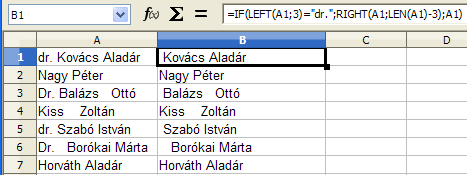
\includegraphics[width=11.354cm]{oocalcv1-img90.png}
\caption{18. feladat}\label{18-feladat}
\end{center}
\end{figure}

Figyeljük meg a kifejezés struktúráját a
Függvénytündér ablakában (\ref{18-feladatIF} ábra). Több beágyazott
függvény használatakor a kifejezés működését segít
megérteni, ha kiválasztjuk valamelyik beágyazott függvényt
és megvizsgáljuk argumentumait és eredményét.

\begin{figure}[!h]
\begin{center}
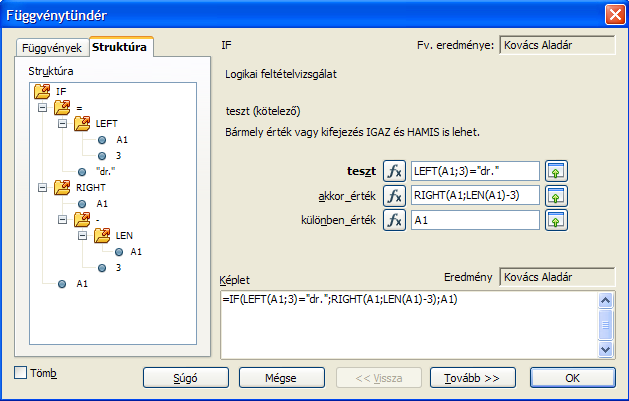
\includegraphics[width=15.999cm]{oocalcv1-img91.png}
\caption{18. feladat --  Függvénytündér -- IF kifejezés struktúra}\label{18-feladatIF}
\end{center}
\end{figure}

A nevekből távolítsuk el a fölösleges szóköz
karaktereket. Az eddigi kifejezés legyen a TRIM függvény
argumentuma. A feladat megoldása \aref{18-feladatMegoldás} ábrán látható.

\begin{figure}[!h]
\begin{center}
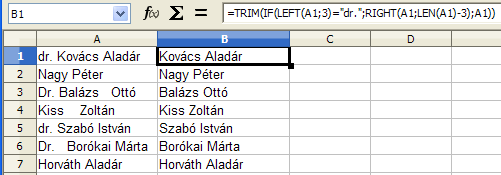
\includegraphics[width=12.254cm]{oocalcv1-img92.png}
\caption{18. feladat -- Megoldás}\label{18-feladatMegoldás}
\end{center}
\end{figure}

Jól látható, hogy mind a vezeték-, mind a keresztnév elé
beírt szóközökből csak egy maradt a B oszlopban.

A \textbf{\&} operátor, amivel szövegeket kapcsolhatunk össze,
segítségünkre lehet számítási feladatok esetén is.
Vizsgáljuk meg ezt a következő feladatban.


\clearpage
\section{19. feladat}

{\itshape
Határozzuk meg, hogy a 12. feladatban vizsgált osztály tanulói
közül hányan értek az osztályátlag fölötti átlagot.}

A feladat megoldására a COUNTIF függvényt nem tudjuk alapesetben
használni, hiszen a függvény második feltétel argumentuma nem
lehet sem függvény, sem hivatkozás. Még visszatérünk ehhez
a függvényhez, de először oldjuk meg a feladatot logikai
függvények és segédoszlop felhasználásával. Másoljuk a
12. feladat A1:I10 tartományát egy üres munkalapra. A J2
cellába pedig írjuk a következő kifejezést:
\textsf{\textbf{=IF(I2>AVERAGE(D\$2:H\$10);1;0)}}.
Ez a cella 1-et fog felvenni, ha az első tanuló átlaga az
osztályátlagnál jobb, és 0-át, ha rosszabb. A képletet
másolva számoszlopot kapunk, aminek összege megadja a keresett
eredményt (\ref{19-feladat} ábra).

\begin{figure}[!h]
\begin{center}
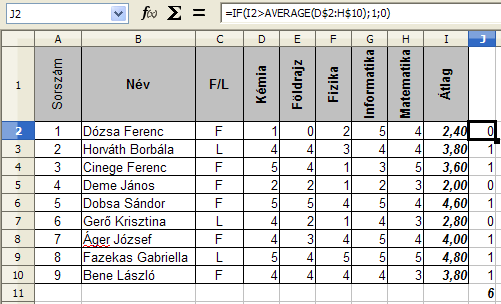
\includegraphics[width=13.254cm]{oocalcv1-img93.png}
\caption{19. feladat}\label{19-feladat}
\end{center}
\end{figure}

A COUNTIF függvény második argumentumában a \textbf{\&}
operátort felhasználva a következő kifejezéssel adhatjuk
meg a feltétel argumentumot:
\textsf{\textbf{">"\&AVERAGE(D2:H10))}}.
A végleges képlet tehát:
\textsf{\textbf{=COUNTIF(I2:I10;">"\&AVERAGE(D2:H10))}}.
Írjuk be a képletet a J12 cellába és ellenőrizzük, hogy
ugyanazt az eredményt adja mint az előző esetben.

Az ebben a fejezetben áttekintett függvényeket
\aref{9-fejezetFüggvények} táblázatban találjuk meg.


\begin{table}[!h]
\begin{center}
\caption{A fejezetben tárgyalt függvények}\label{9-fejezetFüggvények}
\begin{tabular}{|m{3cm}|m{8cm}|m{3cm}|}
\hline
 & & \multicolumn{1}{c|}{\textbf{Megfelelője a}} \\
\multicolumn{1}{|c|}{\textbf{A függvény}}&
\multicolumn{1}{c|}{\textbf{Funkciója}}&
\multicolumn{1}{c|}{\textbf{magyar}} \\
\multicolumn{1}{|c|}{\textbf{neve}} & &
\multicolumn{1}{c|}{\textbf{Microsoft}} \\
 & & \multicolumn{1}{c|}{\textbf{Excelben}} \\
\hline
CONCATENATE & Karakterláncokat egyesít. & ÖSSZEFŰZ\\ \hline
EXACT & Összehasonlít két szöveges karakterláncot. & AZONOS\\ \hline
SEARCH & Egy szövegrész karakterláncon belüli helyzetét adja eredményül.
Kis és nagybetűk között nem tesz különbséget. & SZÖVEG.KERES\\ \hline
FIND & Egy szövegrész karakterláncon belüli helyzetét adja
eredményül. Kis és nagybetűk között különbséget tesz. & SZÖVEG.TALÁL\\ \hline
LEFT & Megadja egy szöveg első karaktereit. & BAL\\ \hline
RIGHT & Megadja egy szöveg utolsó karaktereit. & JOBB\\ \hline
MID & Megadja egy karakterlánc egy darabját. & KÖZÉP\\ \hline
LEN & Szöveg karaktereinek számát adja. & HOSSZ\\ \hline
LOWER & Kisbetűsre alakítja a szöveget. & KISBETŰ\\ \hline
UPPER & Nagybetűsre alakítja a szöveget. & NAGYBETŰS\\ \hline
SUBSTITUTE & Megadott karaktereket cserél szövegben. & HELYETTE\\ \hline
REPLACE & Karaktereket cserél szövegben pozíció alapján. & CSERE\\ \hline
TEXT & Megadott formátum alapján számot szöveggé alakít. & SZÖVEG\\ \hline
TRIM & Eltávolítja a szükségtelen szóközöket. & TRIM\\ \hline
ROMAN & Római számra alakít. & RÓMAI\\ \hline
ARABIC & Római számot arab számmá alakít. & {}-\\ \hline
VALUE & Szöveget számmá alakít. & ÉRTÉK\\ \hline
\end{tabular}
\end{center}
\end{table}

